\subsection{Methodology}
\begin{frame}
    \frametitle{Fuel cycle simulators}
    To quantify potential material needs, we can model the transition 
    from the current \gls{LWR} fleet to advanced reactors
    \begin{itemize}
        \item Use fuel cycle simulators to model the transition
        \item Model the deployment and decommissioning of fuel cycle facilities 
        \item Model material transactions between facilities
        \item Quantify material requirements to understand potential \gls{HALEU}
              demand
    \end{itemize}
    For this work, I am using \Cyclus \cite{huff_fundamental_2016}

\end{frame}

\begin{frame}
    \frametitle{Transition analysis assumptions}
    \begin{columns}
        
    \column[t]{6cm}
    \vspace{-0.9cm}
    \begin{figure}[t]
    \centering
    \begin{tikzpicture}[node distance=1cm]
        \node (mine) [agent] {Uranium Mine};
        \node (enrichment) [agent, below of=mine]{Enrichment};
        \node (reactor) [agent, below of=enrichment]{LWR};
        \node (adv_reactor) [transition, below of=enrichment, xshift=2cm]{Advanced Reactor};
        \node (wetstorage) [agent, below of=reactor]{Wet Storage};
        \node (sinkhlw) [agent, below of=wetstorage, xshift=0.75cm]{Repository};
        \node (sinkllw) [agent, left of=enrichment,xshift=-1cm]{Tails Sink};
        \node (adv_rx_cooling) [transition, below of=adv_reactor]{Wet Storage};

        \draw [arrow] (mine) --  (enrichment); 
        \draw [arrow] (enrichment) -- (sinkllw);
        \draw [arrow] (enrichment) -- (reactor);
        \draw [arrow] (enrichment) -- (adv_reactor);
        \draw [arrow] (reactor) -- (wetstorage);
        \draw [arrow] (wetstorage) -- (sinkhlw);
        \draw [arrow] (adv_reactor) -- (adv_rx_cooling);
        \draw [arrow] (adv_rx_cooling) -- (sinkhlw);
        \end{tikzpicture}
    \caption{Fuel cycle facilities and material flow between facilities. Facilities 
    in red are deployed at the start of the transition. }
    \label{fig:fuel_cycle}
\end{figure}

        \column[t]{4.5cm}
        Provide fuel cycle parameters to \Cyclus
        \begin{itemize}
            \item Simulations model reactor deployment from 1965-2090
            \item Transitions begin in 2025
            \item<2-> \gls{LWR} commission dates are obtained from the IAEA PRIS
                database \cite{noauthor_power_1989}
            \item<2-> \glspl{LWR} are assumed to operate until their current license 
                expires
            \item<3-> Manually calculate advanced reactor deployment
            \item<3-> Assume natural uranium is enriched to produce all 
                  fuel
        \end{itemize}

\end{columns}
\end{frame}

\begin{frame}
    \frametitle{Advanced reactors}
    \vspace{-0.2cm}
    \begingroup
        \renewcommand{\arraystretch}{1.5}
        \begin{table}
            \small
            \caption{Advanced reactor design specifications}
            \label{tab:reactor_summary}
            \vspace{-0.15cm}
            \begin{tabular}{ l p{1.5cm} p{1.5cm} p{2cm} }
                \hline
                Design Criteria & USNC MMR 
                    \cite{noauthor_usnc_2021} & 
                    X-energy Xe-100 \cite{mulder_overview_2021} & 
                    NuScale VOYGR \cite{nuscale_chapter_2020-1,reyes_nuscale_2021,reyes_correction_2022}\\\hline
                Reactor type & HTGR & HTGR & SMR\\
                Fuel type & UO$_2$ FCM & UCO TRISO & UO$_2$ pellets \\
                Power (MWe) & 5 & 80 & 77\\
                Power (MWth) & 15 & 200 & 250\\
                \tikzmarkin<2->[hl]{a}Enrichment (\% $^{235}U$) & 19.75 & 15.5 & 4.09 \\
                Cycle Length (yr) & 20 & Online & 1.5 \tikzmarkend{a}\\
                Number of cycles & 1 & 6 & 3\\
                Reactor Lifetime (yr) & 20 & 60 & 60\\
                \tikzmarkin<2->[hl]{c}Burnup ($\frac{MWd}{kg U}$) & 82 & 168 & 45\tikzmarkend{c}\\
                \hline
            \end{tabular}
        \end{table}   
    \endgroup
    \begin{equation}
        \text{mass (kg)} = \frac{\text{Power (MWth) * cycle length (d)*number of cycles}}{\text{Burnup (MWd/kg)}}
        \label{eq:fuel_mass}
    \end{equation}
\end{frame}

\begin{frame}
    \frametitle{Once-through scenario definitions}
        \begin{table}[ht]
            \centering
            \caption{Summary of the once-through fuel cycle transition scenarios.
            Energy growth is relative to energy from \glspl{LWR} in 2025.}
            \label{tab:scenarios_once-through}
            \begin{tabular}{c l l}
                \hline
                Scenario number & Reactors present & Energy demand\\\hline
                 1 & \glspl{LWR} & N/A \\
                \tikzmarkin<2->[hl]{b}2 & \glspl{LWR} and MMR & No growth \\
                3 & \glspl{LWR} and Xe-100 & No growth \\
                4 & \glspl{LWR}, Xe-100, and MMR& No growth\\
                5 & \glspl{LWR}, MMR, and VOYGR & No growth\\
                6 & \glspl{LWR}, Xe-100, and VOYGR & No growth\\
                7 & \glspl{LWR}, Xe-100, MMR, and VOYGR & No growth \tikzmarkend{b}\\
                8 & \glspl{LWR} and MMR & 1\% growth \\
                9 & \glspl{LWR} and Xe-100 & 1\% growth \\
                10 & \glspl{LWR}, Xe-100, and MMR& 1\% growth\\
                11 & \glspl{LWR}, MMR, and VOYGR & 1\% growth\\
                12 & \glspl{LWR}, Xe-100, and VOYGR & 1\% growth\\
                13 & \glspl{LWR}, Xe-100, MMR, and VOYGR & 1\% growth\\
                \hline
        \end{tabular}
        \end{table}
        %<2-> \tikz[overlay, remember picture]{\draw{draw=red,thick, double, fillopacity=0.2] ($(infrastructure)+(-0.5,0.4)$) rectangle ($(infrastructure)+(6,-0.2)$);}} 
\end{frame}

\begin{frame}
    \frametitle{Advanced reactor deployment scheme}
    \begin{columns}
        \column[t]{5cm}
            Manually calculate the deployment scheme for advanced reactors
            \begin{itemize}
                \item Preferentially deploy reactors with larger power output first
                \item Deploy reactor with largest power output until an oversupply 
                      of power would be produced, deploy the next reactor until 
                      an oversupply of power, then deploy the last reactor until 
                      demand is met
                \item Deployment schedule is given to \Cyclus
            \end{itemize}
        \column[t]{5.5cm}
            \begin{figure}
                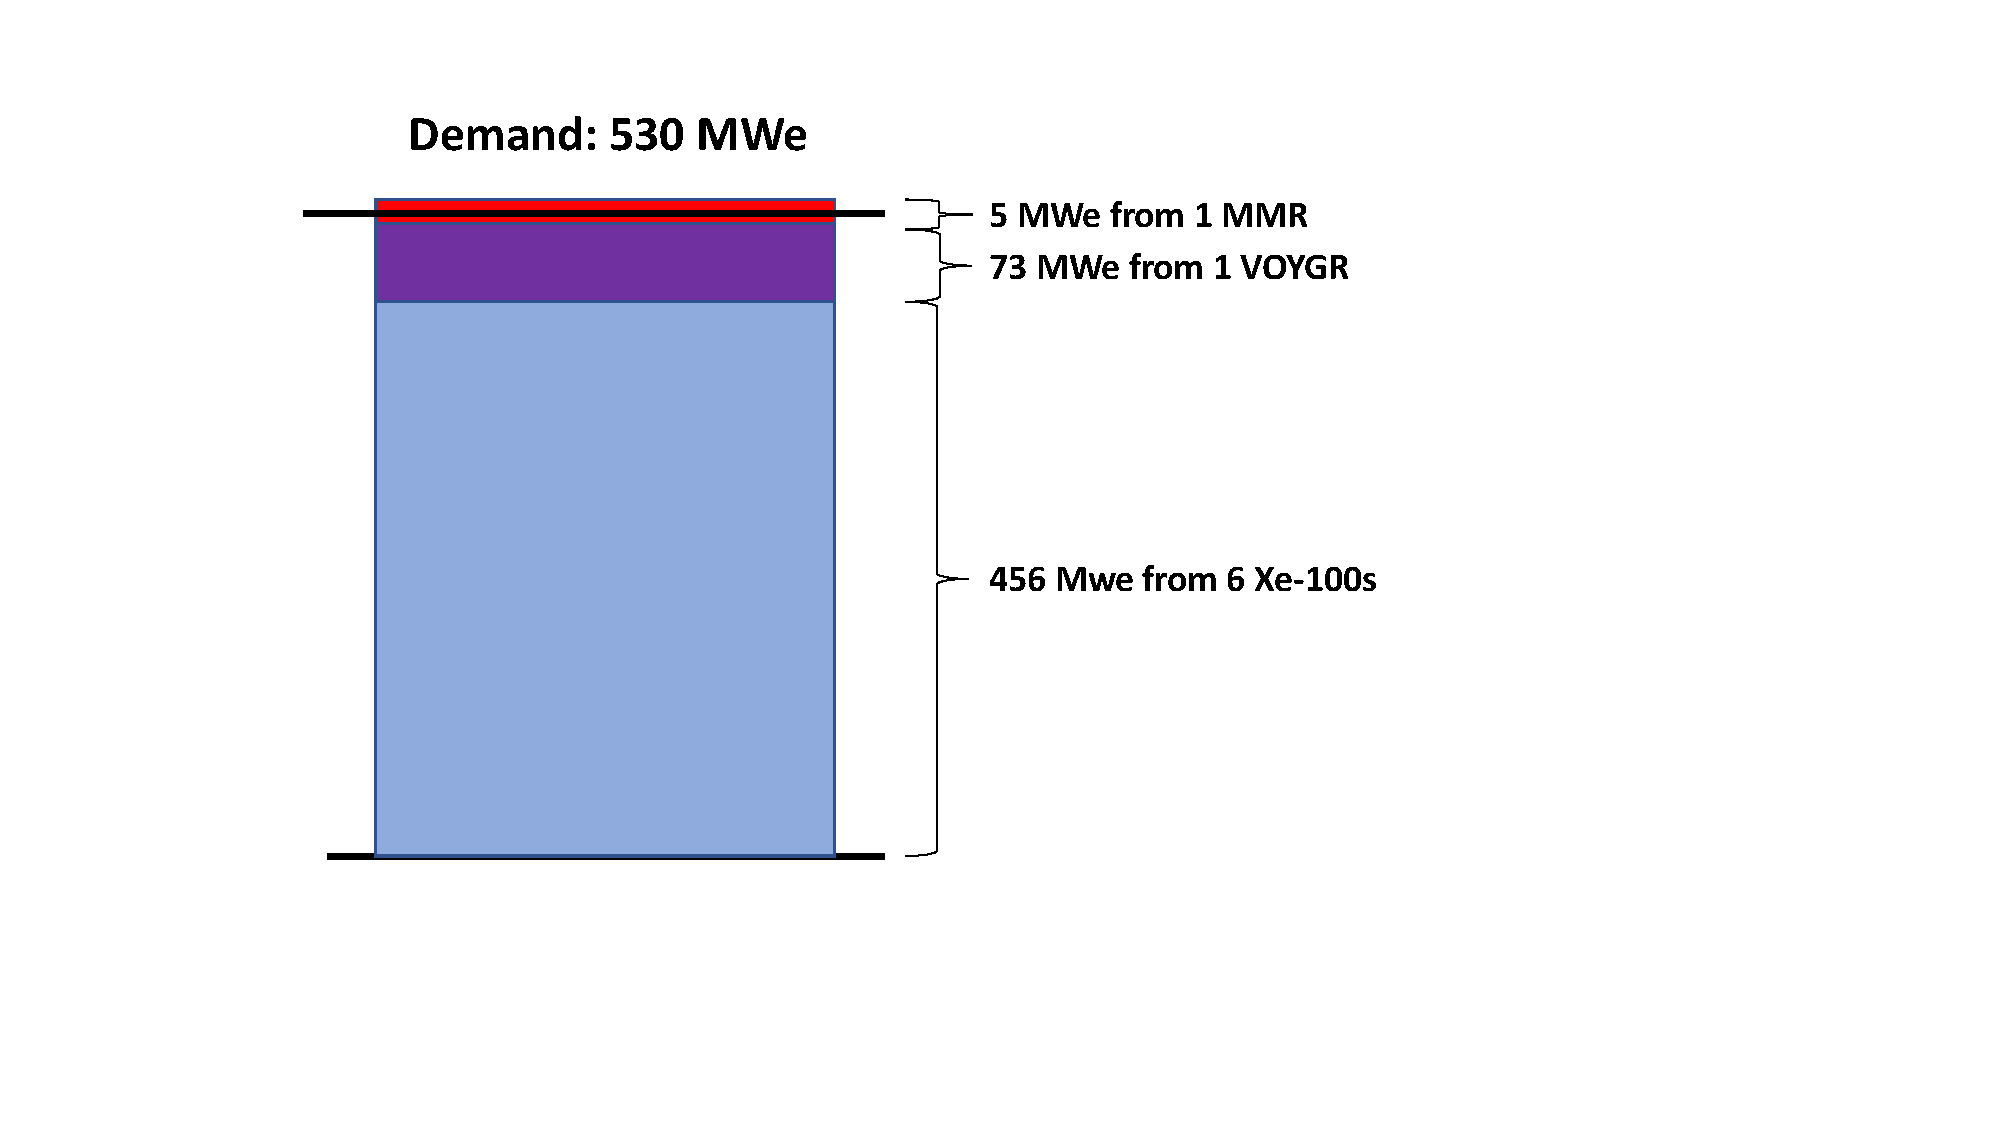
\includegraphics[scale=0.35, trim=150 100 50 50,clip]{Deployment_Scheme.pdf}
                \caption{Example of how advanced reactors in Scenario 7 are deployed to 
                meet a demand of 530 MWe.}
                \label{fig:deployment}
            \end{figure}
                    
    \end{columns}
\end{frame}